 \documentclass{article}
\usepackage[utf8]{inputenc}
\usepackage[a4paper, total={7in, 10in}]{geometry}
\usepackage{braket}
\usepackage{xcolor}
\usepackage{amsmath}
\usepackage{amssymb}
\usepackage{amsfonts}
\usepackage{graphicx}
\usepackage{svg}
\usepackage{float}
\usepackage{tikz}
\usepackage[ruled,vlined]{algorithm2e}
\usepackage{multicol}
\usepackage[backend=biber,style=alphabetic,sorting=ynt]{biblatex}
\usepackage{xcolor}
%\addbibresource{sample.bib} %Import the bibliography file

\newcommand{\commentt}[1]{\textcolor{blue}{ \textbf{[COMMENT]} #1}}
\newcommand{\ctt}[1]{\commentt{#1}}
\newcommand{\prb}[1]{ \mathbf{Pr} \left[ {#1} \right]}
\newcommand{\onotation}[1]{\(\mathcal{O} \left( {#1}  \right) \)}
\newcommand{\ona}[1]{\onotation{#1}}
\newcommand{\PSI}{{\ket{\psi}}}
\newcommand{\LESn}{\ket{\psi_n}}
\newcommand{\LESa}{\ket{\phi_n}}
\newcommand{\LESs}{\frac{1}{\sqrt{n}}\sum_{i}{\ket{\left(0^{i}10^{n-i}\right)^{n}}}}
\newcommand{\Hn}{\mathcal{H}_{n}}
\newcommand{\Ep}{\frac{1}{\sqrt{2^n}}\sum^{2^n}_{x}{ \ket{xx}}}
\newcommand{\HON}{\ket{\psi_{\text{honest}}}}
\newcommand{\Lemma}{\paragraph{Lemma.}}


\setlength{\columnsep}{0.6cm}

\newcommand{\Gz}{ G_{z}^{\delta} } 

\begin{document}

\title{Quantum LTC With Positive Rate}
\author{David Ponarovsky}
\maketitle
%\begin{multicols*}{2}
\newcommand{ \Hw }{ \delta\Delta -\Delta^{\frac{1}{2}-\varepsilon}/\delta  }
	\newcommand{ \Nw }{ \Delta^{\frac{3}{2}-\varepsilon}} 
	  \newcommand{ \Gu } { \Gamma^{\cup} }
	  \newcommand{ \Guq } { \Gamma^{\cup, \square} }

    	\newcommand{ \Gsa } {\Gamma_{\square_{1}} }
	\newcommand{ \Gsb } {\Gamma_{\square_{2}} }
        \newcommand{ \Aa } { C_{A_{1}}}  
	\newcommand{ \Ab } { C_{A_{2}}}
	\newcommand{ \Ac } { C_{A_{3}}}
	\newcommand{ \Aab } { \Aa \otimes \Ab } 
	\newcommand{ \Aac } { \Aa \otimes \Ac }
	\newcommand{ \Aabc } { \Aa \otimes \Ab \otimes \Ac }
	\newcommand{ \Aabp } { \Aa^{\perp} \otimes \Ab^{\perp} } 
	\newcommand{ \Aacp } { \Aa^{\perp} \otimes \Ac^{\perp} }
	\newcommand{ \Aabcp } { \Aa^{\perp} \otimes \Ab^{\perp} \otimes \Ac^{\perp} }
	\newcommand{ \Aabpp } { \left( \Aabp \right)^\perp } 
	\newcommand{ \Aacpp } { \left( \Aacp \right)^\perp }
	\newcommand{ \Aabcpp } { \left( \Aabcp \right)^\perp }
	\newcommand{ \YY } {  y_{1}y_{2}^{\top} }
	\newcommand{ \ZZ } {  z_{1}z_{2}^{\top} } 
	\newcommand{ \TT } { \tilde{\tau} } 


  \paragraph{preamble.} preamble.  
  \begin{figure}[H]
            %\label{fig:square}
            \begin{center}
            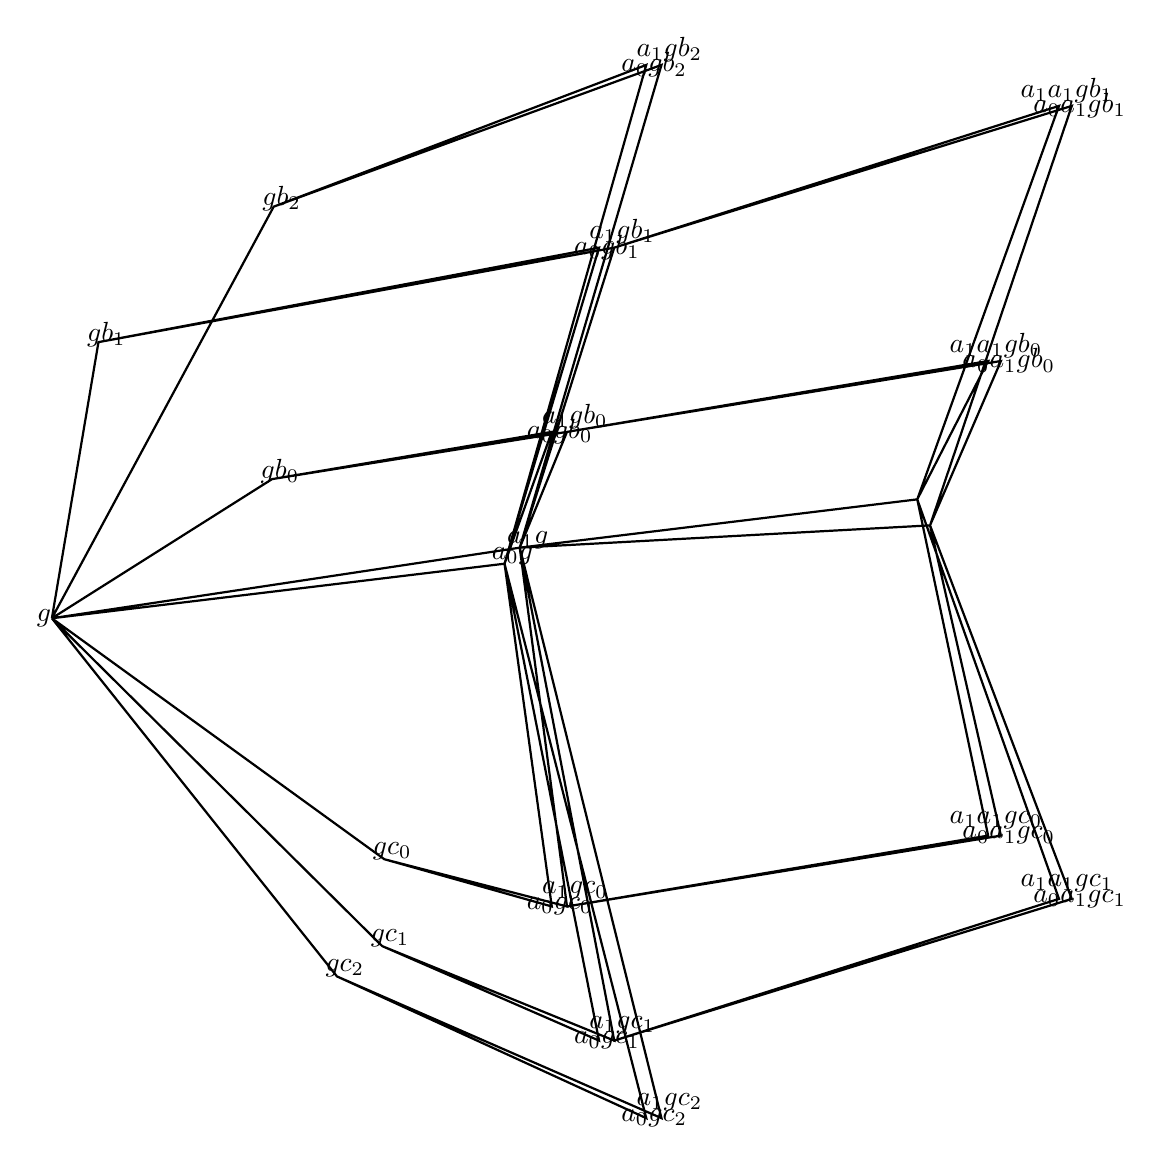
\begin{tikzpicture}
            \draw[thick](0,0)(0, 0) -- (2.7963269713381567,1.7672136574983042) -- (6.348970072469827,2.3672136574983043) -- (5.748970072469827,0.6929568895241923) -- (0, 0)
(0, 0) -- (0.5918942857194182,3.506898829105852) -- (6.948970072469828,4.706898829105852) -- (5.748970072469827,0.6929568895241923) -- (0, 0)
(0, 0) -- (2.8172885243801686,5.227243310841544) -- (7.548970072469827,7.027243310841544) -- (5.748970072469827,0.6929568895241923) -- (0, 0)
(0, 0) -- (2.7963269713381567,1.7672136574983042) -- (6.542126309942735,2.3672136574983043) -- (5.9421263099427355,0.8966178250118034) -- (0, 0)
(0, 0) -- (0.5918942857194182,3.506898829105852) -- (7.142126309942736,4.706898829105852) -- (5.9421263099427355,0.8966178250118034) -- (0, 0)
(0, 0) -- (2.8172885243801686,5.227243310841544) -- (7.742126309942735,7.027243310841544) -- (5.9421263099427355,0.8966178250118034) -- (0, 0)
(0, 0) -- (4.221821614065248,-3.0600051144845066) -- (6.348970072469827,-3.6600051144845067) -- (5.748970072469827,0.6929568895241923) -- (0, 0)
(0, 0) -- (4.194882838074448,-4.163393221437312) -- (6.948970072469828,-5.363393221437312) -- (5.748970072469827,0.6929568895241923) -- (0, 0)
(0, 0) -- (3.6208094008116665,-4.548454210683534) -- (7.548970072469827,-6.348454210683534) -- (5.748970072469827,0.6929568895241923) -- (0, 0)
(0, 0) -- (4.221821614065248,-3.0600051144845066) -- (6.542126309942735,-3.6600051144845067) -- (5.9421263099427355,0.8966178250118034) -- (0, 0)
(0, 0) -- (4.194882838074448,-4.163393221437312) -- (7.142126309942736,-5.363393221437312) -- (5.9421263099427355,0.8966178250118034) -- (0, 0)
(0, 0) -- (3.6208094008116665,-4.548454210683534) -- (7.742126309942735,-6.348454210683534) -- (5.9421263099427355,0.8966178250118034) -- (0, 0)
(5.9421263099427355, 0.8966178250118034) -- (6.542126309942735,2.3672136574983043) -- (12.05277046661862,3.267213657498304) -- (11.15277046661862,1.1798227772035033) -- (5.9421263099427355, 0.8966178250118034)
(5.9421263099427355, 0.8966178250118034) -- (7.142126309942736,4.706898829105852) -- (12.95277046661862,6.506898829105852) -- (11.15277046661862,1.1798227772035033) -- (5.9421263099427355, 0.8966178250118034)
(5.9421263099427355, 0.8966178250118034) -- (6.542126309942735,2.3672136574983043) -- (11.890372839351462,3.267213657498304) -- (10.990372839351462,1.5100365825731785) -- (5.9421263099427355, 0.8966178250118034)
(5.9421263099427355, 0.8966178250118034) -- (7.142126309942736,4.706898829105852) -- (12.790372839351463,6.506898829105852) -- (10.990372839351462,1.5100365825731785) -- (5.9421263099427355, 0.8966178250118034)
(5.9421263099427355, 0.8966178250118034) -- (6.542126309942735,-3.6600051144845067) -- (12.05277046661862,-2.760005114484507) -- (11.15277046661862,1.1798227772035033) -- (5.9421263099427355, 0.8966178250118034)
(5.9421263099427355, 0.8966178250118034) -- (7.142126309942736,-5.363393221437312) -- (12.95277046661862,-3.5633932214373125) -- (11.15277046661862,1.1798227772035033) -- (5.9421263099427355, 0.8966178250118034)
(5.9421263099427355, 0.8966178250118034) -- (6.542126309942735,-3.6600051144845067) -- (11.890372839351462,-2.760005114484507) -- (10.990372839351462,1.5100365825731785) -- (5.9421263099427355, 0.8966178250118034)
(5.9421263099427355, 0.8966178250118034) -- (7.142126309942736,-5.363393221437312) -- (12.790372839351463,-3.5633932214373125) -- (10.990372839351462,1.5100365825731785) -- (5.9421263099427355, 0.8966178250118034)
;
\node at (6.448970072469827,2.3672136574983043) {$ a_{ 0  } gb_{ 0 } $};
\node at (7.048970072469827,4.706898829105852) {$ a_{ 0  } gb_{ 1 } $};
\node at (7.648970072469827,7.027243310841544) {$ a_{ 0  } gb_{ 2 } $};
\node at (6.642126309942735,2.5672136574983044) {$ a_{ 1  } gb_{ 0 } $};
\node at (7.242126309942735,4.906898829105852) {$ a_{ 1  } gb_{ 1 } $};
\node at (7.842126309942735,7.227243310841544) {$ a_{ 1  } gb_{ 2 } $};
\node at (6.448970072469827,-3.6600051144845067) {$ a_{ 0  } gc_{ 0 } $};
\node at (7.048970072469827,-5.363393221437312) {$ a_{ 0  } gc_{ 1 } $};
\node at (7.648970072469827,-6.348454210683534) {$ a_{ 0  } gc_{ 2 } $};
\node at (6.642126309942735,-3.4600051144845065) {$ a_{ 1  } gc_{ 0 } $};
\node at (7.242126309942735,-5.163393221437312) {$ a_{ 1  } gc_{ 1 } $};
\node at (7.842126309942735,-6.148454210683534) {$ a_{ 1  } gc_{ 2 } $};
\node at (12.15277046661862,3.267213657498304) {$ a_{ 0  } a_{ 1 }gb_{ 0 } $};
\node at (13.05277046661862,6.506898829105852) {$ a_{ 0  } a_{ 1 }gb_{ 1 } $};
\node at (11.990372839351462,3.4672136574983043) {$ a_{ 1  } a_{ 1 }gb_{ 0 } $};
\node at (12.890372839351462,6.706898829105852) {$ a_{ 1  } a_{ 1 }gb_{ 1 } $};
\node at (12.15277046661862,-2.760005114484507) {$ a_{ 0  } a_{ 1 }gc_{ 0 } $};
\node at (13.05277046661862,-3.5633932214373125) {$ a_{ 0  } a_{ 1 }gc_{ 1 } $};
\node at (11.990372839351462,-2.5600051144845066) {$ a_{ 1  } a_{ 1 }gc_{ 0 } $};
\node at (12.890372839351462,-3.3633932214373123) {$ a_{ 1  } a_{ 1 }gc_{ 1 } $};
\node at (-0.1,0) {$ g $};
\node at (5.848970072469827,0.7929568895241923) {$ a_{ 0 }g $};
\node at (6.042126309942735,0.9966178250118034) {$ a_{ 1 }g $};
\node at (2.8963269713381568,1.8672136574983043) {$ gb_{ 0 } $};
\node at (0.6918942857194181,3.606898829105852) {$ gb_{ 1 } $};
\node at (2.9172885243801687,5.327243310841544) {$ gb_{ 2 } $};
\node at (4.3218216140652475,-2.9600051144845065) {$ gc_{ 0 } $};
\node at (4.2948828380744475,-4.0633932214373125) {$ gc_{ 1 } $};
\node at (3.7208094008116666,-4.4484542106835345) {$ gc_{ 2 } $};

            \end{tikzpicture}
            \end{center}
            \caption{Square of the complex, with edges $(g,ag), (agb, gb) \in E_A,
            (g,gb), (agb, ag) \in E_B.$ \label{fig:square}
            }
            \end{figure}
 \begin{figure}[H]
            %\label{fig:square}
            \begin{center}
            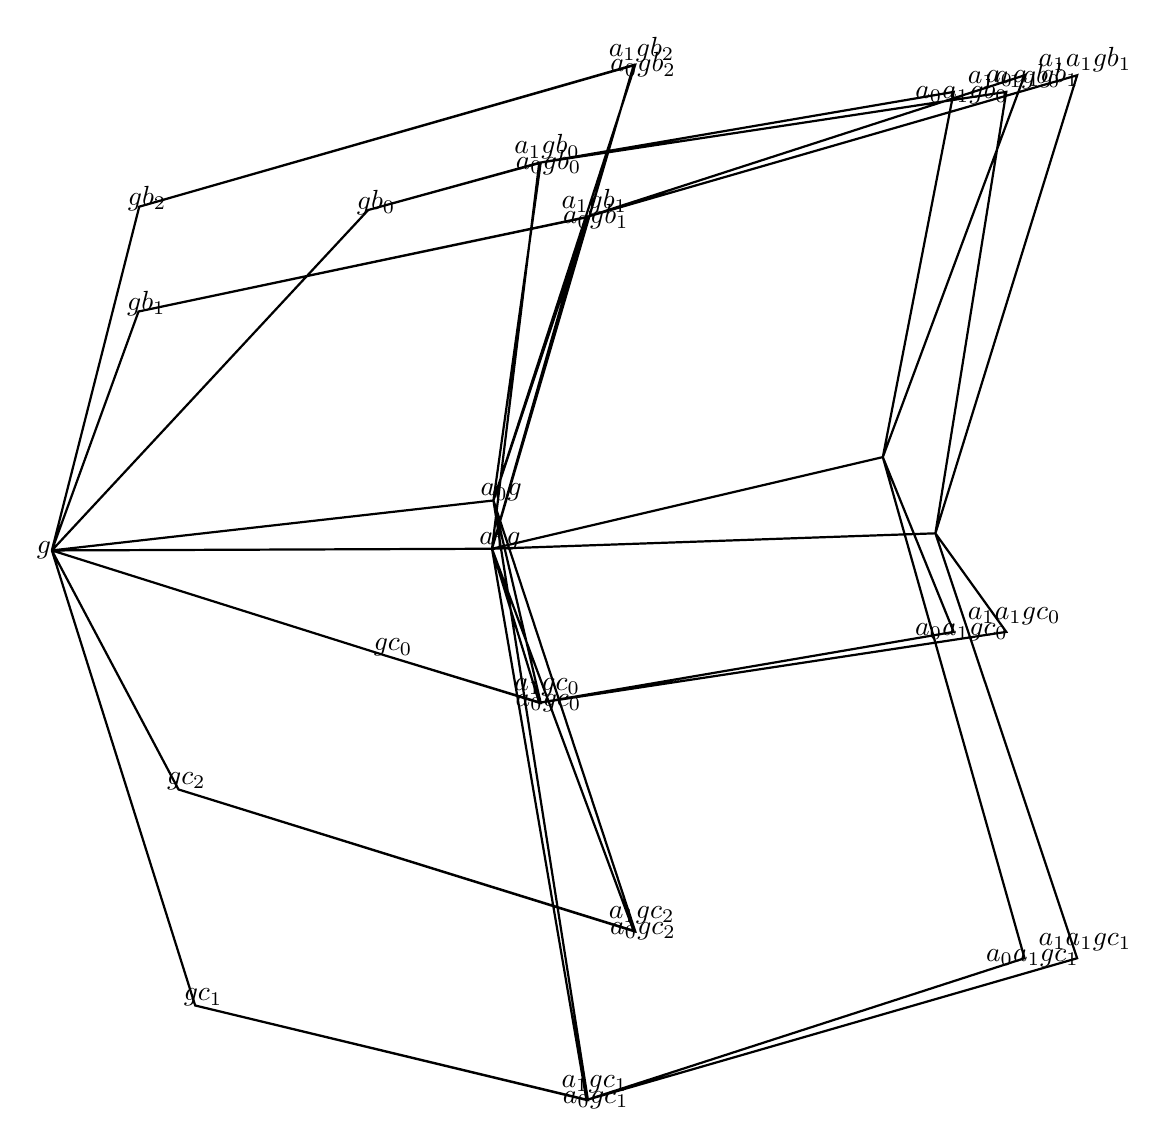
\begin{tikzpicture}
            \draw[thick](0,0)(0, 0) -- (4.017720501501333,4.3234433161694845) -- (6.207858500831307,4.923443316169484) -- (5.607858500831307,0.6344686001266416) -- (0, 0)
(0, 0) -- (1.1007782436777864,3.0343543429002757) -- (6.8078585008313075,4.234354342900276) -- (5.607858500831307,0.6344686001266416) -- (0, 0)
(0, 0) -- (1.1097797875552162,4.365832470146727) -- (7.407858500831307,6.165832470146727) -- (5.607858500831307,0.6344686001266416) -- (0, 0)
(0, 0) -- (4.017720501501333,4.3234433161694845) -- (6.189680937149758,4.923443316169484) -- (5.589680937149758,0.02146063726018399) -- (0, 0)
(0, 0) -- (1.1007782436777864,3.0343543429002757) -- (6.789680937149758,4.234354342900276) -- (5.589680937149758,0.02146063726018399) -- (0, 0)
(0, 0) -- (1.1097797875552162,4.365832470146727) -- (7.389680937149758,6.165832470146727) -- (5.589680937149758,0.02146063726018399) -- (0, 0)
(0, 0) -- (4.233137078324826,-1.3342350933160847) -- (6.207858500831307,-1.9342350933160848) -- (5.607858500831307,0.6344686001266416) -- (0, 0)
(0, 0) -- (1.819923444562872,-5.778943995737018) -- (6.8078585008313075,-6.978943995737018) -- (5.607858500831307,0.6344686001266416) -- (0, 0)
(0, 0) -- (1.607944660930749,-3.035443794643441) -- (7.407858500831307,-4.8354437946434405) -- (5.607858500831307,0.6344686001266416) -- (0, 0)
(0, 0) -- (4.233137078324826,-1.3342350933160847) -- (6.189680937149758,-1.9342350933160848) -- (5.589680937149758,0.02146063726018399) -- (0, 0)
(0, 0) -- (1.819923444562872,-5.778943995737018) -- (6.789680937149758,-6.978943995737018) -- (5.589680937149758,0.02146063726018399) -- (0, 0)
(0, 0) -- (1.607944660930749,-3.035443794643441) -- (7.389680937149758,-4.8354437946434405) -- (5.589680937149758,0.02146063726018399) -- (0, 0)
(5.589680937149758, 0.02146063726018399) -- (6.189680937149758,4.923443316169484) -- (11.453056328782564,5.8234433161694845) -- (10.553056328782564,1.185414144100849) -- (5.589680937149758, 0.02146063726018399)
(5.589680937149758, 0.02146063726018399) -- (6.789680937149758,4.234354342900276) -- (12.353056328782564,6.034354342900276) -- (10.553056328782564,1.185414144100849) -- (5.589680937149758, 0.02146063726018399)
(5.589680937149758, 0.02146063726018399) -- (6.189680937149758,4.923443316169484) -- (12.120803586318113,5.8234433161694845) -- (11.220803586318112,0.21733923983167217) -- (5.589680937149758, 0.02146063726018399)
(5.589680937149758, 0.02146063726018399) -- (6.789680937149758,4.234354342900276) -- (13.020803586318113,6.034354342900276) -- (11.220803586318112,0.21733923983167217) -- (5.589680937149758, 0.02146063726018399)
(5.589680937149758, 0.02146063726018399) -- (6.189680937149758,-1.9342350933160848) -- (11.453056328782564,-1.0342350933160849) -- (10.553056328782564,1.185414144100849) -- (5.589680937149758, 0.02146063726018399)
(5.589680937149758, 0.02146063726018399) -- (6.789680937149758,-6.978943995737018) -- (12.353056328782564,-5.1789439957370185) -- (10.553056328782564,1.185414144100849) -- (5.589680937149758, 0.02146063726018399)
(5.589680937149758, 0.02146063726018399) -- (6.189680937149758,-1.9342350933160848) -- (12.120803586318113,-1.0342350933160849) -- (11.220803586318112,0.21733923983167217) -- (5.589680937149758, 0.02146063726018399)
(5.589680937149758, 0.02146063726018399) -- (6.789680937149758,-6.978943995737018) -- (13.020803586318113,-5.1789439957370185) -- (11.220803586318112,0.21733923983167217) -- (5.589680937149758, 0.02146063726018399)
;
\node at (6.307858500831307,4.923443316169484) {$ a_{ 0  } gb_{ 0 } $};
\node at (6.907858500831307,4.234354342900276) {$ a_{ 0  } gb_{ 1 } $};
\node at (7.507858500831307,6.165832470146727) {$ a_{ 0  } gb_{ 2 } $};
\node at (6.2896809371497575,5.123443316169484) {$ a_{ 1  } gb_{ 0 } $};
\node at (6.889680937149758,4.434354342900276) {$ a_{ 1  } gb_{ 1 } $};
\node at (7.489680937149758,6.365832470146727) {$ a_{ 1  } gb_{ 2 } $};
\node at (6.307858500831307,-1.9342350933160848) {$ a_{ 0  } gc_{ 0 } $};
\node at (6.907858500831307,-6.978943995737018) {$ a_{ 0  } gc_{ 1 } $};
\node at (7.507858500831307,-4.8354437946434405) {$ a_{ 0  } gc_{ 2 } $};
\node at (6.2896809371497575,-1.7342350933160848) {$ a_{ 1  } gc_{ 0 } $};
\node at (6.889680937149758,-6.778943995737018) {$ a_{ 1  } gc_{ 1 } $};
\node at (7.489680937149758,-4.63544379464344) {$ a_{ 1  } gc_{ 2 } $};
\node at (11.553056328782564,5.8234433161694845) {$ a_{ 0  } a_{ 1 }gb_{ 0 } $};
\node at (12.453056328782564,6.034354342900276) {$ a_{ 0  } a_{ 1 }gb_{ 1 } $};
\node at (12.220803586318112,6.023443316169485) {$ a_{ 1  } a_{ 1 }gb_{ 0 } $};
\node at (13.120803586318113,6.234354342900276) {$ a_{ 1  } a_{ 1 }gb_{ 1 } $};
\node at (11.553056328782564,-1.0342350933160849) {$ a_{ 0  } a_{ 1 }gc_{ 0 } $};
\node at (12.453056328782564,-5.1789439957370185) {$ a_{ 0  } a_{ 1 }gc_{ 1 } $};
\node at (12.220803586318112,-0.8342350933160849) {$ a_{ 1  } a_{ 1 }gc_{ 0 } $};
\node at (13.120803586318113,-4.978943995737018) {$ a_{ 1  } a_{ 1 }gc_{ 1 } $};
\node at (-0.1,0) {$ g $};
\node at (5.707858500831307,0.7344686001266416) {$ a_{ 0 }g $};
\node at (5.689680937149758,0.121460637260184) {$ a_{ 1 }g $};
\node at (4.117720501501332,4.423443316169484) {$ gb_{ 0 } $};
\node at (1.2007782436777865,3.134354342900276) {$ gb_{ 1 } $};
\node at (1.2097797875552163,4.465832470146727) {$ gb_{ 2 } $};
\node at (4.3331370783248255,-1.2342350933160846) {$ gc_{ 0 } $};
\node at (1.9199234445628721,-5.6789439957370185) {$ gc_{ 1 } $};
\node at (1.7079446609307491,-2.935443794643441) {$ gc_{ 2 } $};

            \end{tikzpicture}
            \end{center}
            \caption{Square of the complex, with edges $(g,ag), (agb, gb) \in E_A,
            (g,gb), (agb, ag) \in E_B.$ \label{fig:square}
            }
            \end{figure}
 \begin{figure}[H]
            %\label{fig:square}
            \begin{center}
            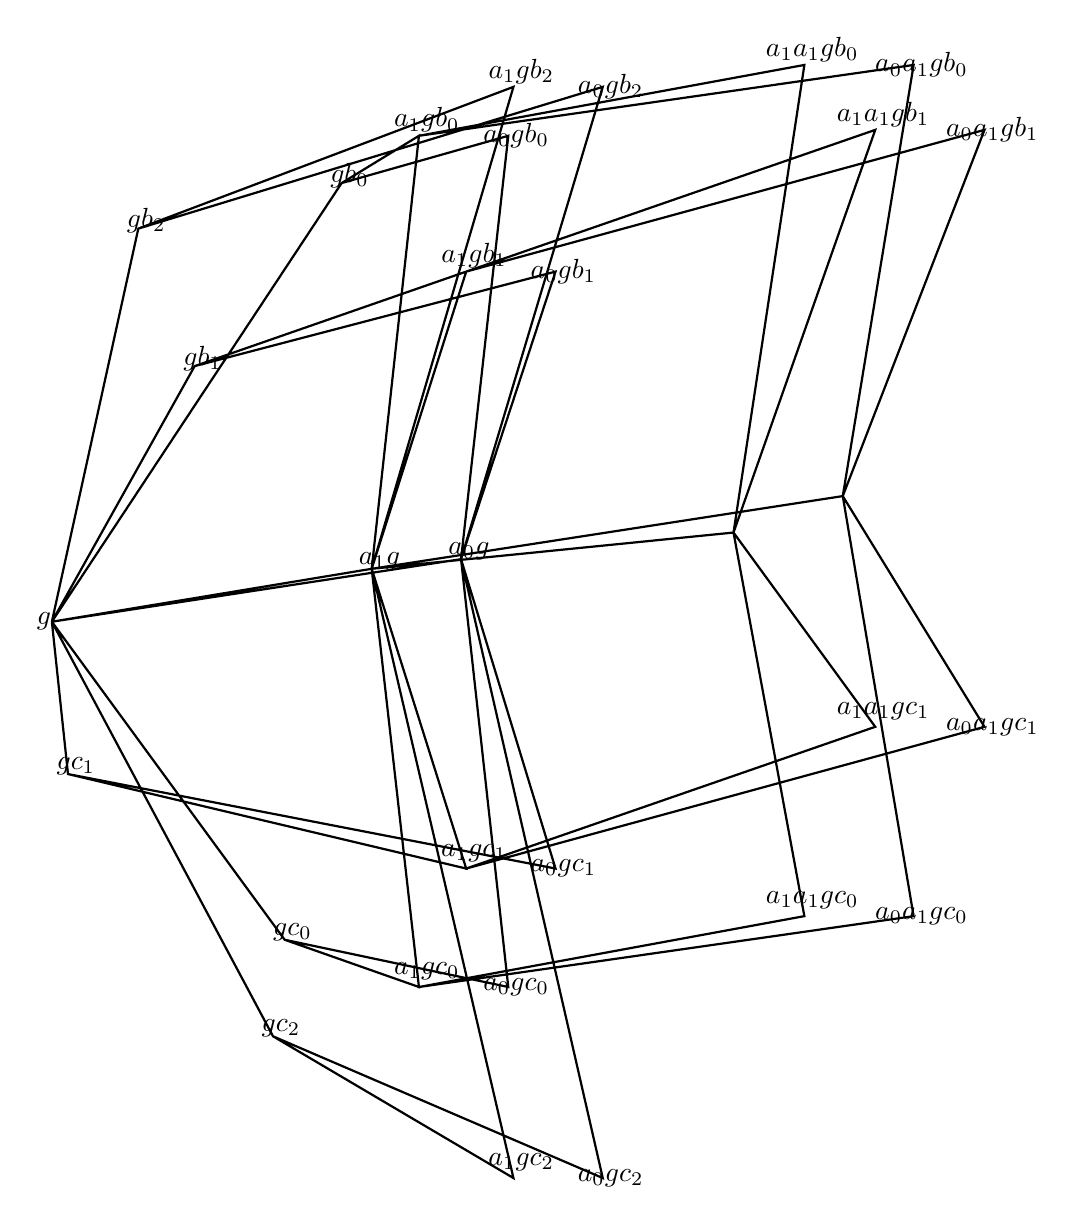
\begin{tikzpicture}
            \draw[thick](0,0)(0, 0) -- (3.680303752761488,5.571188411114722) -- (5.796388626528253,6.171188411114722) -- (5.196388626528253,0.7946570161736684) -- (0, 0)
(0, 0) -- (1.813693381188466,3.2465156815987264) -- (6.396388626528253,4.446515681598727) -- (5.196388626528253,0.7946570161736684) -- (0, 0)
(0, 0) -- (1.0978883441738507,4.9926919984646645) -- (6.996388626528253,6.792691998464664) -- (5.196388626528253,0.7946570161736684) -- (0, 0)
(0, 0) -- (3.680303752761488,5.571188411114722) -- (4.661821663244792,6.171188411114722) -- (4.0618216632447925,0.6721303320495167) -- (0, 0)
(0, 0) -- (1.813693381188466,3.2465156815987264) -- (5.261821663244793,4.446515681598727) -- (4.0618216632447925,0.6721303320495167) -- (0, 0)
(0, 0) -- (1.0978883441738507,4.9926919984646645) -- (5.861821663244792,6.792691998464664) -- (4.0618216632447925,0.6721303320495167) -- (0, 0)
(0, 0) -- (2.956215787781816,-4.038883011805363) -- (5.796388626528253,-4.638883011805363) -- (5.196388626528253,0.7946570161736684) -- (0, 0)
(0, 0) -- (0.20473449011304656,-1.934501863034514) -- (6.396388626528253,-3.1345018630345143) -- (5.196388626528253,0.7946570161736684) -- (0, 0)
(0, 0) -- (2.8087276119728797,-5.265016261880328) -- (6.996388626528253,-7.065016261880328) -- (5.196388626528253,0.7946570161736684) -- (0, 0)
(0, 0) -- (2.956215787781816,-4.038883011805363) -- (4.661821663244792,-4.638883011805363) -- (4.0618216632447925,0.6721303320495167) -- (0, 0)
(0, 0) -- (0.20473449011304656,-1.934501863034514) -- (5.261821663244793,-3.1345018630345143) -- (4.0618216632447925,0.6721303320495167) -- (0, 0)
(0, 0) -- (2.8087276119728797,-5.265016261880328) -- (5.861821663244792,-7.065016261880328) -- (4.0618216632447925,0.6721303320495167) -- (0, 0)
(4.0618216632447925, 0.6721303320495167) -- (4.661821663244792,6.171188411114722) -- (10.944235906712636,7.071188411114722) -- (10.044235906712636,1.5955255540473503) -- (4.0618216632447925, 0.6721303320495167)
(4.0618216632447925, 0.6721303320495167) -- (5.261821663244793,4.446515681598727) -- (11.844235906712637,6.246515681598726) -- (10.044235906712636,1.5955255540473503) -- (4.0618216632447925, 0.6721303320495167)
(4.0618216632447925, 0.6721303320495167) -- (4.661821663244792,6.171188411114722) -- (9.556834291815932,7.071188411114722) -- (8.656834291815931,1.1326813735026728) -- (4.0618216632447925, 0.6721303320495167)
(4.0618216632447925, 0.6721303320495167) -- (5.261821663244793,4.446515681598727) -- (10.456834291815932,6.246515681598726) -- (8.656834291815931,1.1326813735026728) -- (4.0618216632447925, 0.6721303320495167)
(4.0618216632447925, 0.6721303320495167) -- (4.661821663244792,-4.638883011805363) -- (10.944235906712636,-3.738883011805363) -- (10.044235906712636,1.5955255540473503) -- (4.0618216632447925, 0.6721303320495167)
(4.0618216632447925, 0.6721303320495167) -- (5.261821663244793,-3.1345018630345143) -- (11.844235906712637,-1.3345018630345142) -- (10.044235906712636,1.5955255540473503) -- (4.0618216632447925, 0.6721303320495167)
(4.0618216632447925, 0.6721303320495167) -- (4.661821663244792,-4.638883011805363) -- (9.556834291815932,-3.738883011805363) -- (8.656834291815931,1.1326813735026728) -- (4.0618216632447925, 0.6721303320495167)
(4.0618216632447925, 0.6721303320495167) -- (5.261821663244793,-3.1345018630345143) -- (10.456834291815932,-1.3345018630345142) -- (8.656834291815931,1.1326813735026728) -- (4.0618216632447925, 0.6721303320495167)
;
\node at (5.896388626528252,6.171188411114722) {$ a_{ 0  } gb_{ 0 } $};
\node at (6.496388626528253,4.446515681598727) {$ a_{ 0  } gb_{ 1 } $};
\node at (7.0963886265282525,6.792691998464664) {$ a_{ 0  } gb_{ 2 } $};
\node at (4.761821663244792,6.371188411114722) {$ a_{ 1  } gb_{ 0 } $};
\node at (5.361821663244792,4.646515681598727) {$ a_{ 1  } gb_{ 1 } $};
\node at (5.961821663244792,6.9926919984646645) {$ a_{ 1  } gb_{ 2 } $};
\node at (5.896388626528252,-4.638883011805363) {$ a_{ 0  } gc_{ 0 } $};
\node at (6.496388626528253,-3.1345018630345143) {$ a_{ 0  } gc_{ 1 } $};
\node at (7.0963886265282525,-7.065016261880328) {$ a_{ 0  } gc_{ 2 } $};
\node at (4.761821663244792,-4.438883011805363) {$ a_{ 1  } gc_{ 0 } $};
\node at (5.361821663244792,-2.934501863034514) {$ a_{ 1  } gc_{ 1 } $};
\node at (5.961821663244792,-6.865016261880328) {$ a_{ 1  } gc_{ 2 } $};
\node at (11.044235906712636,7.071188411114722) {$ a_{ 0  } a_{ 1 }gb_{ 0 } $};
\node at (11.944235906712636,6.246515681598726) {$ a_{ 0  } a_{ 1 }gb_{ 1 } $};
\node at (9.656834291815931,7.271188411114722) {$ a_{ 1  } a_{ 1 }gb_{ 0 } $};
\node at (10.556834291815932,6.446515681598727) {$ a_{ 1  } a_{ 1 }gb_{ 1 } $};
\node at (11.044235906712636,-3.738883011805363) {$ a_{ 0  } a_{ 1 }gc_{ 0 } $};
\node at (11.944235906712636,-1.3345018630345142) {$ a_{ 0  } a_{ 1 }gc_{ 1 } $};
\node at (9.656834291815931,-3.5388830118053627) {$ a_{ 1  } a_{ 1 }gc_{ 0 } $};
\node at (10.556834291815932,-1.1345018630345143) {$ a_{ 1  } a_{ 1 }gc_{ 1 } $};
\node at (-0.1,0) {$ g $};
\node at (5.296388626528253,0.8946570161736683) {$ a_{ 0 }g $};
\node at (4.161821663244792,0.7721303320495166) {$ a_{ 1 }g $};
\node at (3.7803037527614882,5.671188411114722) {$ gb_{ 0 } $};
\node at (1.913693381188466,3.3465156815987265) {$ gb_{ 1 } $};
\node at (1.1978883441738508,5.092691998464664) {$ gb_{ 2 } $};
\node at (3.056215787781816,-3.938883011805363) {$ gc_{ 0 } $};
\node at (0.30473449011304654,-1.834501863034514) {$ gc_{ 1 } $};
\node at (2.9087276119728798,-5.165016261880329) {$ gc_{ 2 } $};

            \end{tikzpicture}
            \end{center}
            \caption{Square of the complex, with edges $(g,ag), (agb, gb) \in E_A,
            (g,gb), (agb, ag) \in E_B.$ \label{fig:square}
            }
            \end{figure}
 \begin{figure}[H]
            %\label{fig:square}
            \begin{center}
            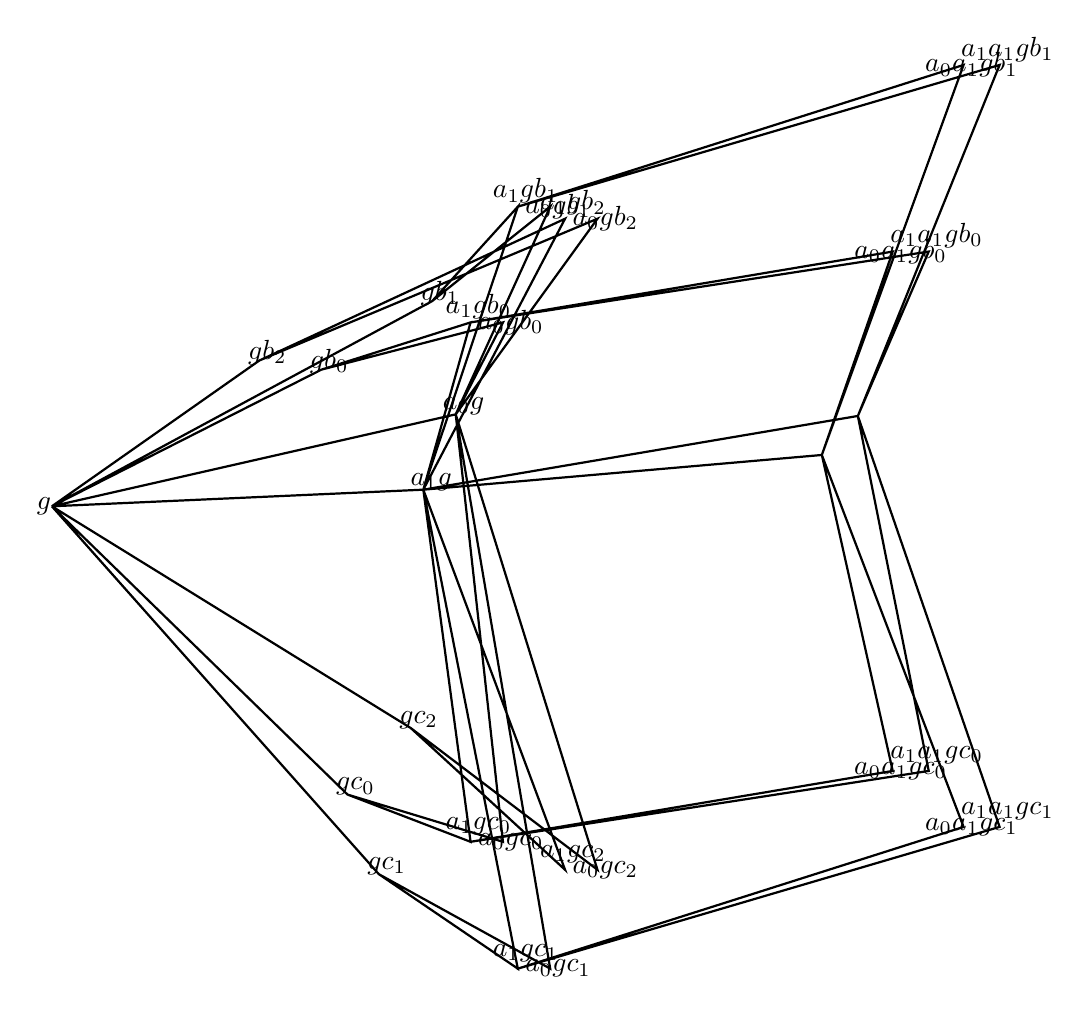
\begin{tikzpicture}
            \draw[thick](0,0)(0, 0) -- (3.422311419405331,1.7350946357634442) -- (5.728862640517369,2.3350946357634443) -- (5.12886264051737,1.1676819729927832) -- (0, 0)
(0, 0) -- (4.828844755039618,2.6050580315151066) -- (6.32886264051737,3.805058031515107) -- (5.12886264051737,1.1676819729927832) -- (0, 0)
(0, 0) -- (2.6359750405085935,1.8519116745295214) -- (6.928862640517369,3.6519116745295213) -- (5.12886264051737,1.1676819729927832) -- (0, 0)
(0, 0) -- (3.422311419405331,1.7350946357634442) -- (5.317409566802994,2.3350946357634443) -- (4.717409566802995,0.2108992301592047) -- (0, 0)
(0, 0) -- (4.828844755039618,2.6050580315151066) -- (5.917409566802995,3.805058031515107) -- (4.717409566802995,0.2108992301592047) -- (0, 0)
(0, 0) -- (2.6359750405085935,1.8519116745295214) -- (6.5174095668029945,3.6519116745295213) -- (4.717409566802995,0.2108992301592047) -- (0, 0)
(0, 0) -- (3.7549097884756346,-3.6610207846235845) -- (5.728862640517369,-4.261020784623584) -- (5.12886264051737,1.1676819729927832) -- (0, 0)
(0, 0) -- (4.152358006254308,-4.671941183394044) -- (6.32886264051737,-5.8719411833940445) -- (5.12886264051737,1.1676819729927832) -- (0, 0)
(0, 0) -- (4.557624539945635,-2.8160994520499765) -- (6.928862640517369,-4.616099452049976) -- (5.12886264051737,1.1676819729927832) -- (0, 0)
(0, 0) -- (3.7549097884756346,-3.6610207846235845) -- (5.317409566802994,-4.261020784623584) -- (4.717409566802995,0.2108992301592047) -- (0, 0)
(0, 0) -- (4.152358006254308,-4.671941183394044) -- (5.917409566802995,-5.8719411833940445) -- (4.717409566802995,0.2108992301592047) -- (0, 0)
(0, 0) -- (4.557624539945635,-2.8160994520499765) -- (6.5174095668029945,-4.616099452049976) -- (4.717409566802995,0.2108992301592047) -- (0, 0)
(4.717409566802995, 0.2108992301592047) -- (5.317409566802994,2.3350946357634443) -- (10.67867508862708,3.2350946357634442) -- (9.778675088627079,0.6516269789843889) -- (4.717409566802995, 0.2108992301592047)
(4.717409566802995, 0.2108992301592047) -- (5.917409566802995,3.805058031515107) -- (11.57867508862708,5.605058031515107) -- (9.778675088627079,0.6516269789843889) -- (4.717409566802995, 0.2108992301592047)
(4.717409566802995, 0.2108992301592047) -- (5.317409566802994,2.3350946357634443) -- (11.135971681042866,3.2350946357634442) -- (10.235971681042866,1.14707261549672) -- (4.717409566802995, 0.2108992301592047)
(4.717409566802995, 0.2108992301592047) -- (5.917409566802995,3.805058031515107) -- (12.035971681042867,5.605058031515107) -- (10.235971681042866,1.14707261549672) -- (4.717409566802995, 0.2108992301592047)
(4.717409566802995, 0.2108992301592047) -- (5.317409566802994,-4.261020784623584) -- (10.67867508862708,-3.3610207846235842) -- (9.778675088627079,0.6516269789843889) -- (4.717409566802995, 0.2108992301592047)
(4.717409566802995, 0.2108992301592047) -- (5.917409566802995,-5.8719411833940445) -- (11.57867508862708,-4.071941183394045) -- (9.778675088627079,0.6516269789843889) -- (4.717409566802995, 0.2108992301592047)
(4.717409566802995, 0.2108992301592047) -- (5.317409566802994,-4.261020784623584) -- (11.135971681042866,-3.3610207846235842) -- (10.235971681042866,1.14707261549672) -- (4.717409566802995, 0.2108992301592047)
(4.717409566802995, 0.2108992301592047) -- (5.917409566802995,-5.8719411833940445) -- (12.035971681042867,-4.071941183394045) -- (10.235971681042866,1.14707261549672) -- (4.717409566802995, 0.2108992301592047)
;
\node at (5.828862640517369,2.3350946357634443) {$ a_{ 0  } gb_{ 0 } $};
\node at (6.428862640517369,3.805058031515107) {$ a_{ 0  } gb_{ 1 } $};
\node at (7.028862640517369,3.6519116745295213) {$ a_{ 0  } gb_{ 2 } $};
\node at (5.417409566802994,2.5350946357634445) {$ a_{ 1  } gb_{ 0 } $};
\node at (6.0174095668029945,4.005058031515107) {$ a_{ 1  } gb_{ 1 } $};
\node at (6.617409566802994,3.8519116745295214) {$ a_{ 1  } gb_{ 2 } $};
\node at (5.828862640517369,-4.261020784623584) {$ a_{ 0  } gc_{ 0 } $};
\node at (6.428862640517369,-5.8719411833940445) {$ a_{ 0  } gc_{ 1 } $};
\node at (7.028862640517369,-4.616099452049976) {$ a_{ 0  } gc_{ 2 } $};
\node at (5.417409566802994,-4.061020784623584) {$ a_{ 1  } gc_{ 0 } $};
\node at (6.0174095668029945,-5.671941183394044) {$ a_{ 1  } gc_{ 1 } $};
\node at (6.617409566802994,-4.416099452049976) {$ a_{ 1  } gc_{ 2 } $};
\node at (10.778675088627079,3.2350946357634442) {$ a_{ 0  } a_{ 1 }gb_{ 0 } $};
\node at (11.67867508862708,5.605058031515107) {$ a_{ 0  } a_{ 1 }gb_{ 1 } $};
\node at (11.235971681042866,3.4350946357634444) {$ a_{ 1  } a_{ 1 }gb_{ 0 } $};
\node at (12.135971681042866,5.805058031515107) {$ a_{ 1  } a_{ 1 }gb_{ 1 } $};
\node at (10.778675088627079,-3.3610207846235842) {$ a_{ 0  } a_{ 1 }gc_{ 0 } $};
\node at (11.67867508862708,-4.071941183394045) {$ a_{ 0  } a_{ 1 }gc_{ 1 } $};
\node at (11.235971681042866,-3.161020784623584) {$ a_{ 1  } a_{ 1 }gc_{ 0 } $};
\node at (12.135971681042866,-3.8719411833940445) {$ a_{ 1  } a_{ 1 }gc_{ 1 } $};
\node at (-0.1,0) {$ g $};
\node at (5.228862640517369,1.2676819729927833) {$ a_{ 0 }g $};
\node at (4.817409566802994,0.31089923015920473) {$ a_{ 1 }g $};
\node at (3.522311419405331,1.8350946357634443) {$ gb_{ 0 } $};
\node at (4.928844755039617,2.7050580315151067) {$ gb_{ 1 } $};
\node at (2.7359750405085936,1.9519116745295215) {$ gb_{ 2 } $};
\node at (3.8549097884756347,-3.5610207846235844) {$ gc_{ 0 } $};
\node at (4.252358006254307,-4.571941183394045) {$ gc_{ 1 } $};
\node at (4.657624539945635,-2.7160994520499764) {$ gc_{ 2 } $};

            \end{tikzpicture}
            \end{center}
            \caption{Square of the complex, with edges $(g,ag), (agb, gb) \in E_A,
            (g,gb), (agb, ag) \in E_B.$ \label{fig:square}
            }
            \end{figure}
 
%\end{multicols*}
  % \printbibliography 
\end{document}

 